\chapter{Аналитический раздел}

\section{Анализ предметной области}

Национальная баскетбольная ассоциация (NBA) является источником одного из наиболее
детализированных массивов спортивной статистики среди крупнейших мировых
профессиональных лиг~\cite{nba-stats}. Для каждого матча фиксируются итоговый
счёт, составы команд и числовые показатели по каждому игроку: очки, подборы,
передачи, блок-шоты, перехваты и иные. На этой основе можно строить рейтинги,
сопоставлять сезоны и выявлять тенденции развития игры.

В современной баскетбольной аналитике для комплексной оценки результативности применяются
продвинутые метрики, стандартизированные в работах ведущих спортивных статистиков~\cite{kubatko}.
Расчёт таких показателей как истинный процент бросков TS\%, эффективный процент с игры eFG\%,
доля владений в атаке USG\%, рейтинг эффективности игрока PER и показатель вклада
игрока BPM требует хранения непротиворечивых первичных данных по матчам, их
агрегирования по сезонам и применения фиксированных правил вычисления.

Обработка спортивной статистики требует строгого контроля над целостностью данных:
сумма очков игроков должна совпадать с командным счётом, агрегаты по сезонам должны
вычисляться из одних и тех же первичных фактов, а параллельный доступ не должен
нарушать консистентность записей. Это определяет необходимость специализированного
хранилища с поддержкой транзакционной целостности и декларативной валидации
бизнес-правил.

\section{Сравнительный анализ существующих систем}

Перед проектированием собственного решения проведём анализ функциональных
возможностей наиболее распространённых публичных систем сбора и анализа
статистики NBA: официального портала NBA Stats~\cite{nba-stats}, справочной
платформы Basketball-Reference~\cite{bref} и аналитического раздела
ESPN~\cite{espn}.

\begin{table}[H]
\centering
\footnotesize
\setlength{\tabcolsep}{3pt}
\renewcommand{\arraystretch}{1.2}
\caption{Сравнительный анализ существующих систем по функциональным возможностям}
\label{tab:systems-compare}
\begin{tabularx}{\textwidth}{|>{\RaggedRight\arraybackslash}p{4.5cm}
  |>{\RaggedRight\centering\arraybackslash}X
  |>{\RaggedRight\centering\arraybackslash}X
  |>{\RaggedRight\centering\arraybackslash}X|}
\hline
\textbf{Критерий} & \textbf{NBA.com Stats} &
\textbf{Basketball-Reference} & \textbf{ESPN Stats} \\
\hline
Просмотр статистики матчей & + & + & + \\
\hline
Фильтрация по сезону, позиции, команде & частично & + & частично \\
\hline
Расчёт TS\%, eFG\%, PER, BPM
  & + (формулы скрыты)
  & + (формулы открыты~\cite{per-bref,myers})
  & частично \\
\hline
Произвольные аналитические запросы & -- & -- & -- \\
\hline
Сравнение игроков & частично & -- & + \\
\hline
Ролевое разграничение доступа & -- & -- & -- \\
\hline
Локальное хранение, воспроизводимость расчётов & -- & -- & -- \\
\hline
\end{tabularx}
\end{table}

Анализ показывает, что NBA.com Stats и ESPN предоставляют данные через готовый
пользовательский интерфейс с непрозрачными формулами расчёта метрик.
Basketball-Reference публикует описание своих формул~\cite{per-bref,myers},
однако не предоставляет открытого API для произвольных аналитических запросов.
Ни одна из систем не поддерживает ролевого разграничения доступа и
воспроизводимого локального хранения данных. Выявленные ограничения определяют
требования к проектируемой системе, сформулированные в следующем разделе.

\section{Требования к проектируемой системе}

\subsection{Функциональные требования}

\begin{enumerate}
    \item хранение справочных данных: игровые позиции, сезоны, клубы NBA;
    \item хранение профилей игроков: персональные и антропометрические данные,
          позиция, сведения о драфте;
    \item хранение данных о матчах: сезон, команды-участники, дата, итоговый
          счёт, статус;
    \item хранение детализированной статистики игрока в матче: очки, подборы,
          передачи, броски с игры и штрафные, потери, фолы, время на площадке;
    \item хранение агрегированной статистики игрока за сезон: средние значения,
          процентные показатели, расчётные метрики;
    \item хранение истории выступлений игрока за клубы по сезонам;
    \item расчёт командной статистики в рамках матча и сезона на основе
          индивидуальных показателей игроков;
    \item автоматизированный расчёт метрик эффективности (eFG\%, TS\%, USG\%,
          PER, BPM) на основе первичных фактов матчей;
    \item предоставление сводных рейтингов игроков и турнирных таблиц команд.
\end{enumerate}

\subsection{Нефункциональные требования}\label{sec:nfr}

\begin{enumerate}
    \item производительность: время отклика на аналитические запросы
          чтения (агрегация за сезон) не должно превышать 200~мс;
    \item объём данных: система должна выдерживать нагрузку не менее
          100\,000 записей в таблице фактов (соответствует статистике за
          5~регулярных сезонов);
    \item целостность: база данных должна соответствовать требованиям
          ACID, обеспечивая ссылочную и логическую целостность на уровне СУБД;
    \item безопасность: ролевое разграничение доступа (администратор,
          аналитик, читатель), реализованное средствами СУБД на уровне таблиц
          и представлений;
    \item масштабируемость чтения: система должна обеспечивать
          кэширование результатов повторяющихся аналитических запросов для
          снижения нагрузки на дисковую подсистему при конкурентном доступе.
\end{enumerate}

\subsection{Ограничения}

\begin{enumerate}
    \item глубина хранения данных ограничена 5~регулярными сезонами
          (с~2019/20 по~2023/24);
    \item пользовательский интерфейс предназначен для просмотра и анализа
          данных, а не для ввода первичной статистики в режиме реального времени.
\end{enumerate}

\section{Метрики эффективности и правила их расчёта}

Обозначения: $\mathrm{PTS}$~--- очки; $\mathrm{FGM}$, $\mathrm{FGA}$~---
попадания и попытки с игры; $\mathrm{FG3M}$~--- трёхочковые; $\mathrm{FTM}$,
$\mathrm{FTA}$~--- штрафные; $\mathrm{TOV}$~--- потери; $\mathrm{TRB}$~---
подборы; $\mathrm{AST}$~--- передачи; $\mathrm{MP}$~--- минуты. Префикс Tm
обозначает командный агрегат по матчам с участием игрока: $\mathrm{TmFGA}$,
$\mathrm{TmFTA}$, $\mathrm{TmTOV}$; $\mathrm{TmMP}$~--- суммарное количество
минут, отыгранных всеми игроками команды в матчах, учитываемых при расчёте
показателя данного игрока.

Командная статистика не выделяется в отдельную сущность: она является
производной от индивидуальных показателей и вычисляется динамически
суммированием по всем игрокам команды в конкретном матче.

\textbf{Эффективный процент с игры, eFG\%}. Метрика корректирует ценность
трёхочкового броска. Согласно методологии NBA~\cite{glossary-nba}, формула имеет вид:
\begin{equation}
\mathrm{eFG\%} = \frac{\mathrm{FGM} + 0{,}5 \cdot \mathrm{FG3M}}{\mathrm{FGA}}
\end{equation}

\textbf{Истинный процент бросков, TS\%}. Показатель объединяет броски с игры и
штрафные броски в единую метрику эффективности. Множитель $0{,}44$ в знаменателе
является эмпирически выведенным коэффициентом Дина Оливера, учитывающим долю
штрафных бросков, завершающих владение~\cite{oliver}:
\begin{equation}
\label{eq:ts}
\mathrm{TS\%} = \frac{\mathrm{PTS}}{2 \cdot (\mathrm{FGA} + 0{,}44 \cdot \mathrm{FTA})}
\end{equation}

\textbf{Доля владений в атаке, USG\%}. Оценивает процент командных владений,
которые завершает конкретный игрок, находясь на площадке~\cite{kubatko}. В базе данных показатель хранится как доля $[0;1]$; в интерфейсе отображается
в процентах ($\times 100$). Формула:
\begin{equation}
\mathrm{USG} =
\frac{(\mathrm{FGA} + 0{,}44 \cdot \mathrm{FTA} + \mathrm{TOV})
      \cdot (\mathrm{TmMP} / 5)}
     {\mathrm{MP} \cdot (\mathrm{TmFGA} + 0{,}44 \cdot
      \mathrm{TmFTA} + \mathrm{TmTOV})}
\end{equation}

Деление $\mathrm{TmMP}$ на~5 нормирует командное время с учётом того, что на
площадке одновременно находятся пять игроков.

\textbf{Рейтинг эффективности игрока, PER}. Оригинальная формула разработана Джоном
Холлинджером~\cite{hollinger}. В настоящей работе применяется её упрощённая версия без
позиционных поправок, методология которой описана на портале Basketball-Reference~\cite{per-bref}.
Подборы $\mathrm{TRB} = \mathrm{REB\_OFF} + \mathrm{REB\_DEF}$.
Ненормализованный вклад приводится к шкале «за 48 минут», затем масштабируется
к среднему по лиге, равному~15:
\begin{equation}
\mathrm{uPER}_i = \Big[\mathrm{PTS} + \mathrm{TRB} + \mathrm{AST} + \mathrm{STL}
+ \mathrm{BLK} - \mathrm{TOV} - \mathrm{PF}
- (\mathrm{FGA} - \mathrm{FGM})
- 0{,}44 \cdot (\mathrm{FTA} - \mathrm{FTM})\Big]
\cdot \frac{48}{\mathrm{MP}_i}
\end{equation}
\begin{equation}
\mathrm{lg\_aPER} = \mathrm{AVG}(\mathrm{uPER}_i)
\quad\text{по игрокам с }\mathrm{MP}_i > 100
\end{equation}
\begin{equation}
\mathrm{PER}_i = \mathrm{uPER}_i \cdot \frac{15}{\mathrm{lg\_aPER}}
\end{equation}

Минимальный порог $\mathrm{MP}_i \ge 50$ минут за сезон; для расчёта
$\mathrm{lg\_aPER}$ учитываются игроки с $\mathrm{MP}_i > 100$ минут.

\textbf{Вклад игрока (Box Plus/Minus, BPM)}. Метрика разработана Дэниелом
Майерсом~\cite{myers}. В системе используется классическая линейная аппроксимация
первой версии алгоритма (BPM 1.0) с нормировкой показателей на 100~минут
($X_{100} = X / \mathrm{MP} \cdot 100$) и учётом
перехватов, блоков и фолов. Итоговая формула:
\begin{equation}
\begin{split}
\mathrm{raw}_i = {}& 0{,}123 \cdot \mathrm{PTS}_{100}
               + 0{,}234 \cdot \mathrm{TRB}_{100}
               + 0{,}689 \cdot \mathrm{AST}_{100}
               + 0{,}445 \cdot \mathrm{STL}_{100} \\
               &{} + 0{,}407 \cdot \mathrm{BLK}_{100}
               - 0{,}605 \cdot \mathrm{TOV}_{100}
               - 0{,}086 \cdot \mathrm{PF}_{100}
\end{split}
\end{equation}
\begin{equation}
\mathrm{BPM}_i = \mathrm{raw}_i - \mathrm{AVG}(\mathrm{raw}_i)
\quad\text{по игрокам с }\mathrm{MP}_i > 100
\end{equation}

Среднее BPM по лиге после вычитания среднего равно~0. Минимальный порог для
расчёта показателя игрока~--- $\mathrm{MP}_i \ge 50$ минут за сезон.

\section{Сущности предметной области, роли пользователей и варианты использования}

\subsection{Сущности и связи}

По результатам анализа предметной области выделены восемь основных сущностей.
\begin{enumerate}
    \item позиция~--- справочник игровых позиций в номенклатуре NBA;
    \item сезон~--- игровой год, его календарные границы и тип турнира;
    \item команда~--- клуб NBA: конференция, дивизион, арена;
    \item игрок~--- персональные и антропометрические данные, позиция,
          сведения о драфте;
    \item матч~--- сезон, команды-участники, дата, счёт, статус;
    \item статистика игрока в матче~--- числовые показатели конкретного
          игрока в конкретной игре; основная таблица фактов предметной области;
    \item статистика игрока за сезон~--- агрегаты и расчётные метрики
          по тройке «игрок~-- сезон~-- команда»;
    \item история выступлений~--- связь «игрок~-- команда~-- сезон»
          с датами и типом контракта.
\end{enumerate}

Связь «многие-ко-многим» между игроками и матчами реализуется через сущность
«Статистика игрока в матче»: один игрок участвует во многих матчах, в одном
матче фиксируется статистика многих игроков~\cite{connolly,chen}.

Связь «Проходит в» на ER-диаграмме является тернарной: она одновременно
связывает сущности «Матч», «Команда» и «Сезон», поскольку матч всегда
привязан к конкретному сезону и двум командам-участницам~\cite{chen}.

Концептуальная ER-диаграмма в нотации Чена приведена на рисунке~\ref{fig:er-chen};
на ней отражены сущности предметной области, бинарные и тернарные связи.

\begin{figure}[H]
\centering
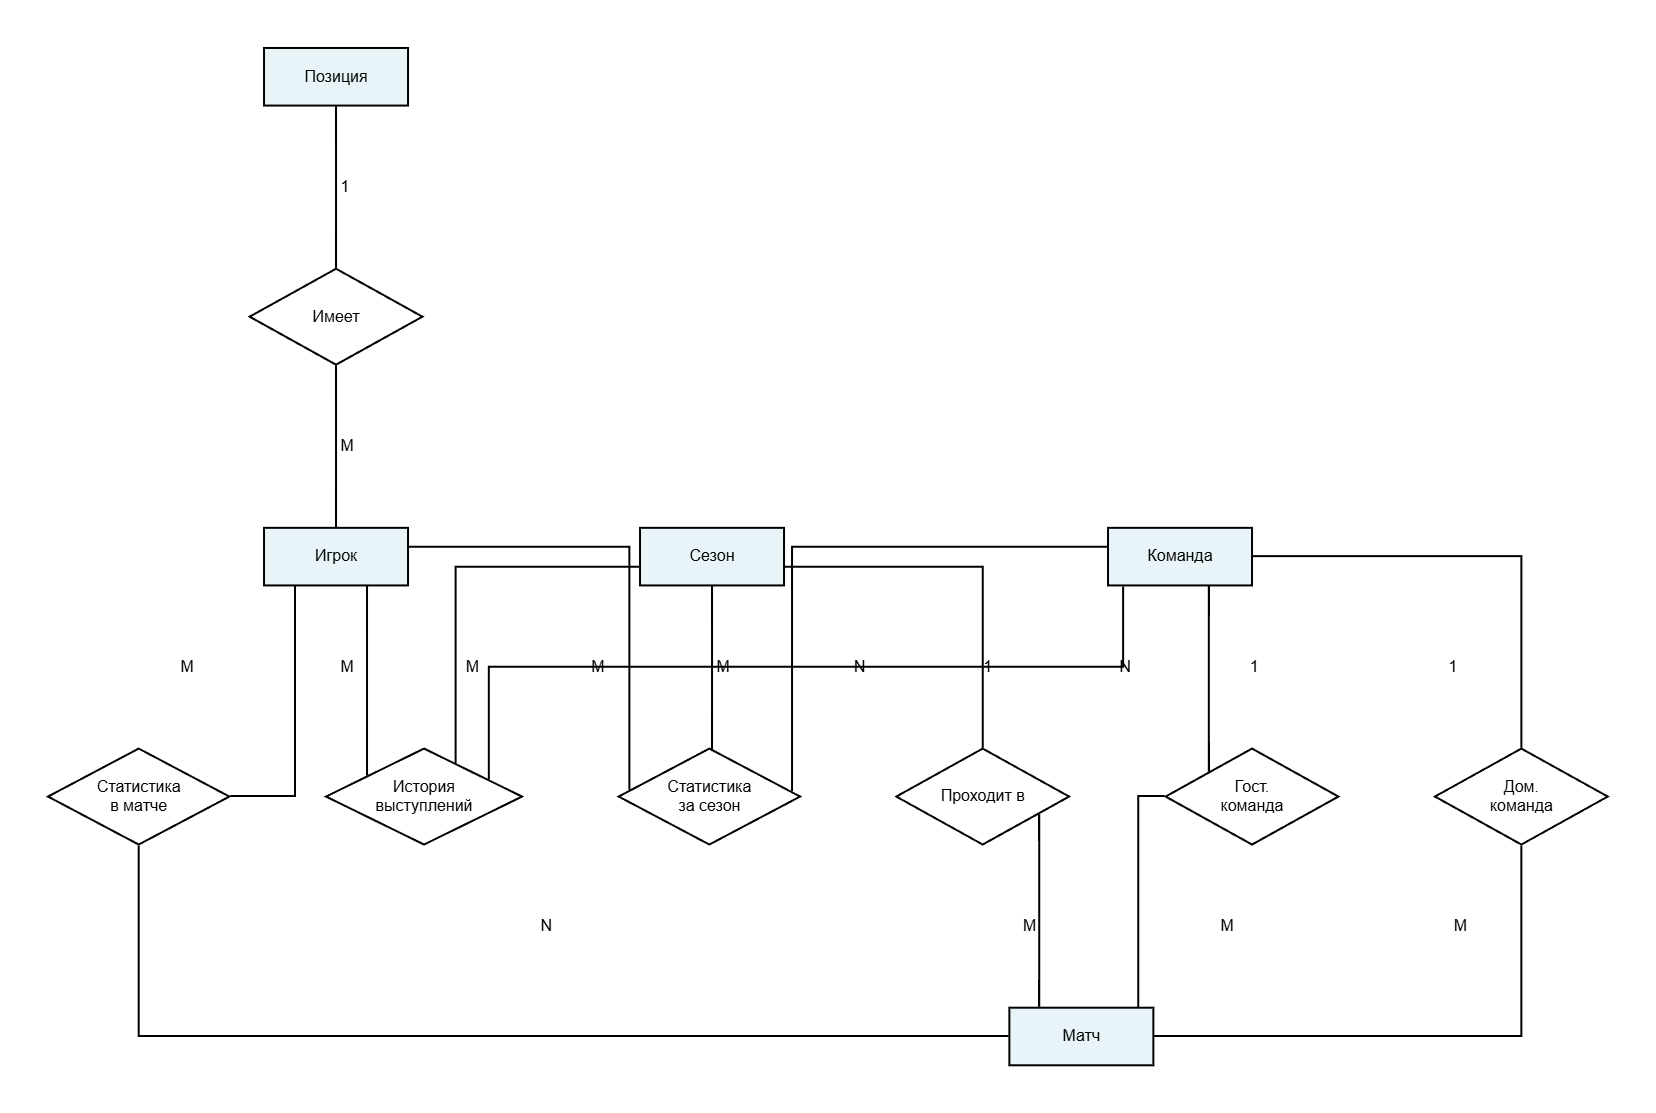
\includegraphics[width=\textwidth]{../img/333.png}
\caption{ER-диаграмма в нотации Чена}
\label{fig:er-chen}
\end{figure}

\subsection{Роли пользователей и варианты использования}\label{sec:use-cases}

Система предусматривает три роли пользователей.
\begin{enumerate}
    \item администратор~--- полное управление структурой и содержимым
          хранилища: создание и изменение схемы, загрузка и сопровождение
          данных, резервное копирование;
    \item аналитик~--- чтение данных и запуск расчётных процедур для
          получения производных показателей;
    \item читатель~--- доступ к агрегированным данным через
          представления; изменение содержимого базовых таблиц недоступно.
\end{enumerate}

Соответствие ролей и допустимых операций задаётся тремя вариантами использования.
\begin{enumerate}
    \item просмотр статистики~--- получение сведений о матчах, игроках
          и командах, агрегированных показателях и рейтингах; доступно всем
          ролям;
    \item расчёт метрик~--- вычисление продвинутых показателей
          (PER, BPM, eFG\%, TS\%, USG\%) на основе первичных данных; доступно
          аналитику и администратору;
    \item управление данными~--- загрузка данных о матчах, обновление
          справочников, изменение схемы; доступно только администратору.
\end{enumerate}

\begin{figure}[H]
\centering
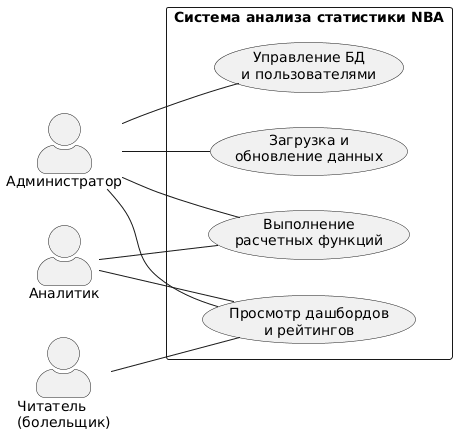
\includegraphics[width=\textwidth]{../img/22.png}
\caption{Диаграмма вариантов использования}
\label{fig:usecase}
\end{figure}

\section{Выбор модели данных}

Для выбора подходящей модели хранения данных проведём сравнение трёх основных
парадигм, опираясь на принципы проектирования дата-интенсивных приложений~\cite{kleppmann}.

\textbf{Документо-ориентированные СУБД (MongoDB, Couchbase)}. Как отмечают
П.~Садаладж и М.~Фаулер~\cite{fowler}, такие базы данных оптимальны для хранения агрегированных
JSON-документов без жёсткой схемы (schema-less). Сырая статистика матча (Box Score)
естественно ложится в документную модель. Однако данный подход существенно
проигрывает в производительности при многомерных агрегациях по нескольким сезонам и не
поддерживает декларативную валидацию бизнес-правил на уровне хранилища.

\textbf{Колоночные СУБД (ClickHouse и аналогичные OLAP-системы)} ориентированы
на аналитику больших объёмов данных: хранение по столбцам многократно ускоряет
агрегирующие запросы (GROUP BY, SUM, AVG)~\cite{clickhouse}. Однако, как указывается
в теории баз данных, OLAP-системы не обеспечивают полноценных транзакций ACID
при смешанных нагрузках, что критично для согласованности данных матчей, и
существенно усложняют реализацию JOIN-запросов между справочниками и таблицами фактов.

\textbf{Реляционные СУБД (PostgreSQL, MySQL)} гарантируют строгую согласованность
данных (ACID) и обладают мощным оптимизатором SQL-запросов~\cite{date}. В отличие
от NoSQL, реляционная модель (schema-on-write) позволяет встроить валидацию
бизнес-логики непосредственно в СУБД через ограничения (CHECK) и триггеры,
что обеспечивает достоверность спортивной статистики.

\begin{table}[H]
\centering
\footnotesize
\setlength{\tabcolsep}{3pt}
\renewcommand{\arraystretch}{1.2}
\caption{Сравнительная характеристика моделей хранения данных}
\label{tab:arch-compare}
\begin{tabularx}{\textwidth}{|>{\RaggedRight\arraybackslash}p{3.2cm}
  |>{\RaggedRight\arraybackslash}X
  |>{\RaggedRight\arraybackslash}X
  |>{\RaggedRight\arraybackslash}X|}
\hline
\textbf{Критерий} & \textbf{Документная СУБД} & \textbf{Колоночная СУБД}
  & \textbf{Реляционная СУБД} \\
\hline
Контроль над схемой & Гибкая (schema-less) & Жёсткая по столбцам
  & Строгая (schema-on-write) \\
\hline
Транзакционность (ACID) & Частичная & Не поддерживается при OLTP-нагрузке
  & Полная \\
\hline
Сложные JOIN-запросы & Затруднены & Затруднены & Встроенная поддержка \\
\hline
Агрегации по сезонам & Средняя (MapReduce) & Высокая (по столбцам)
  & Высокая (оптимизатор SQL) \\
\hline
Валидация бизнес-логики & На уровне приложения & На уровне приложения
  & Встроенная (триггеры, CHECK) \\
\hline
Соответствие структуре матча & Идеальное (JSON) & Требует денормализации
  & Требует декомпозиции \\
\hline
\end{tabularx}
\end{table}

Колоночные СУБД демонстрируют преимущество преимущественно при объёмах от десятков
миллионов строк и строго однородной аналитической нагрузке класса OLAP. Рассматриваемая
система предполагает смешанный профиль использования. Процедура обновления сезонной
статистики выполняет ресурсоёмкие транзакционные операции слияния для сотен записей
одновременно. Кроме того, необходимость ретроспективной корректировки данных из-за
ошибок в официальных протоколах матчей требует гарантированно атомарного обновления
сразу нескольких связанных таблиц.

При целевом объёме таблицы фактов порядка 200\,000 строк классическая реляционная
база данных способна обрабатывать агрегирующие запросы без существенных задержек.
Для наиболее востребованных аналитических выборок, таких как списки лидеров и сводные
турнирные таблицы, применяется кэширование в Redis~\cite{redis}, что полностью
нивелирует отставание в скорости чтения от специализированных аналитических решений.
Использование колоночной СУБД при таком масштабе неизбежно привело бы к усложнению
системы за счёт выделения отдельного транзакционного хранилища для операций записи.
Подобная архитектурная избыточность не даст измеримого выигрыша в производительности.

Таким образом, с учётом требований к транзакционной целостности и предсказуемого
объёма данных, оптимальным выбором является реляционная модель~\cite{date,connolly}.
В качестве основной СУБД выбран PostgreSQL~15~\cite{postgres}.

\section*{Вывод}

Сформулированы функциональные и нефункциональные требования и ограничения;
определён перечень метрик и правила их вычисления. Выделены восемь сущностей,
установлены связи «многие-ко-многим» через таблицы фактов, описаны три
пользовательские роли. По результатам сравнения моделей хранения данных выбрана
реляционная модель (PostgreSQL~15): она единственная обеспечивает полный ACID,
произвольные JOIN-запросы и встроенную валидацию бизнес-логики. Сравнительный
анализ существующих систем (NBA.com Stats, Basketball-Reference, ESPN Stats)
подтвердил отсутствие у них произвольных аналитических запросов, управляемого
ролевого доступа и воспроизводимого локального хранения данных, что
обусловливает целесообразность разработки специализированной базы данных.
Диаграмма вариантов использования и ER-диаграмма приведены на
рисунках~\ref{fig:usecase} и~\ref{fig:er-chen}.